\section{Section 4}

Figure 5 shows that the percentage of services having standards are
increasing over the past few year. For example, among the 1637 services 
available for 2022 to 2023, there were 928 of them with standards, 
representing 56.7\% of the total 2,280 service standards established. Moreover, 
more than 50\% of these service standards were successfully met after 2020, 
indicating an improvement in government performance in meeting service standard 
targets. Notably, during 2022 to 2023, 1,348 out of 2,280 standard targets were 
achieved, accounting for 59.1\%, the highest rate observed in recent years.

\begin{figure}[H]
    \centering
    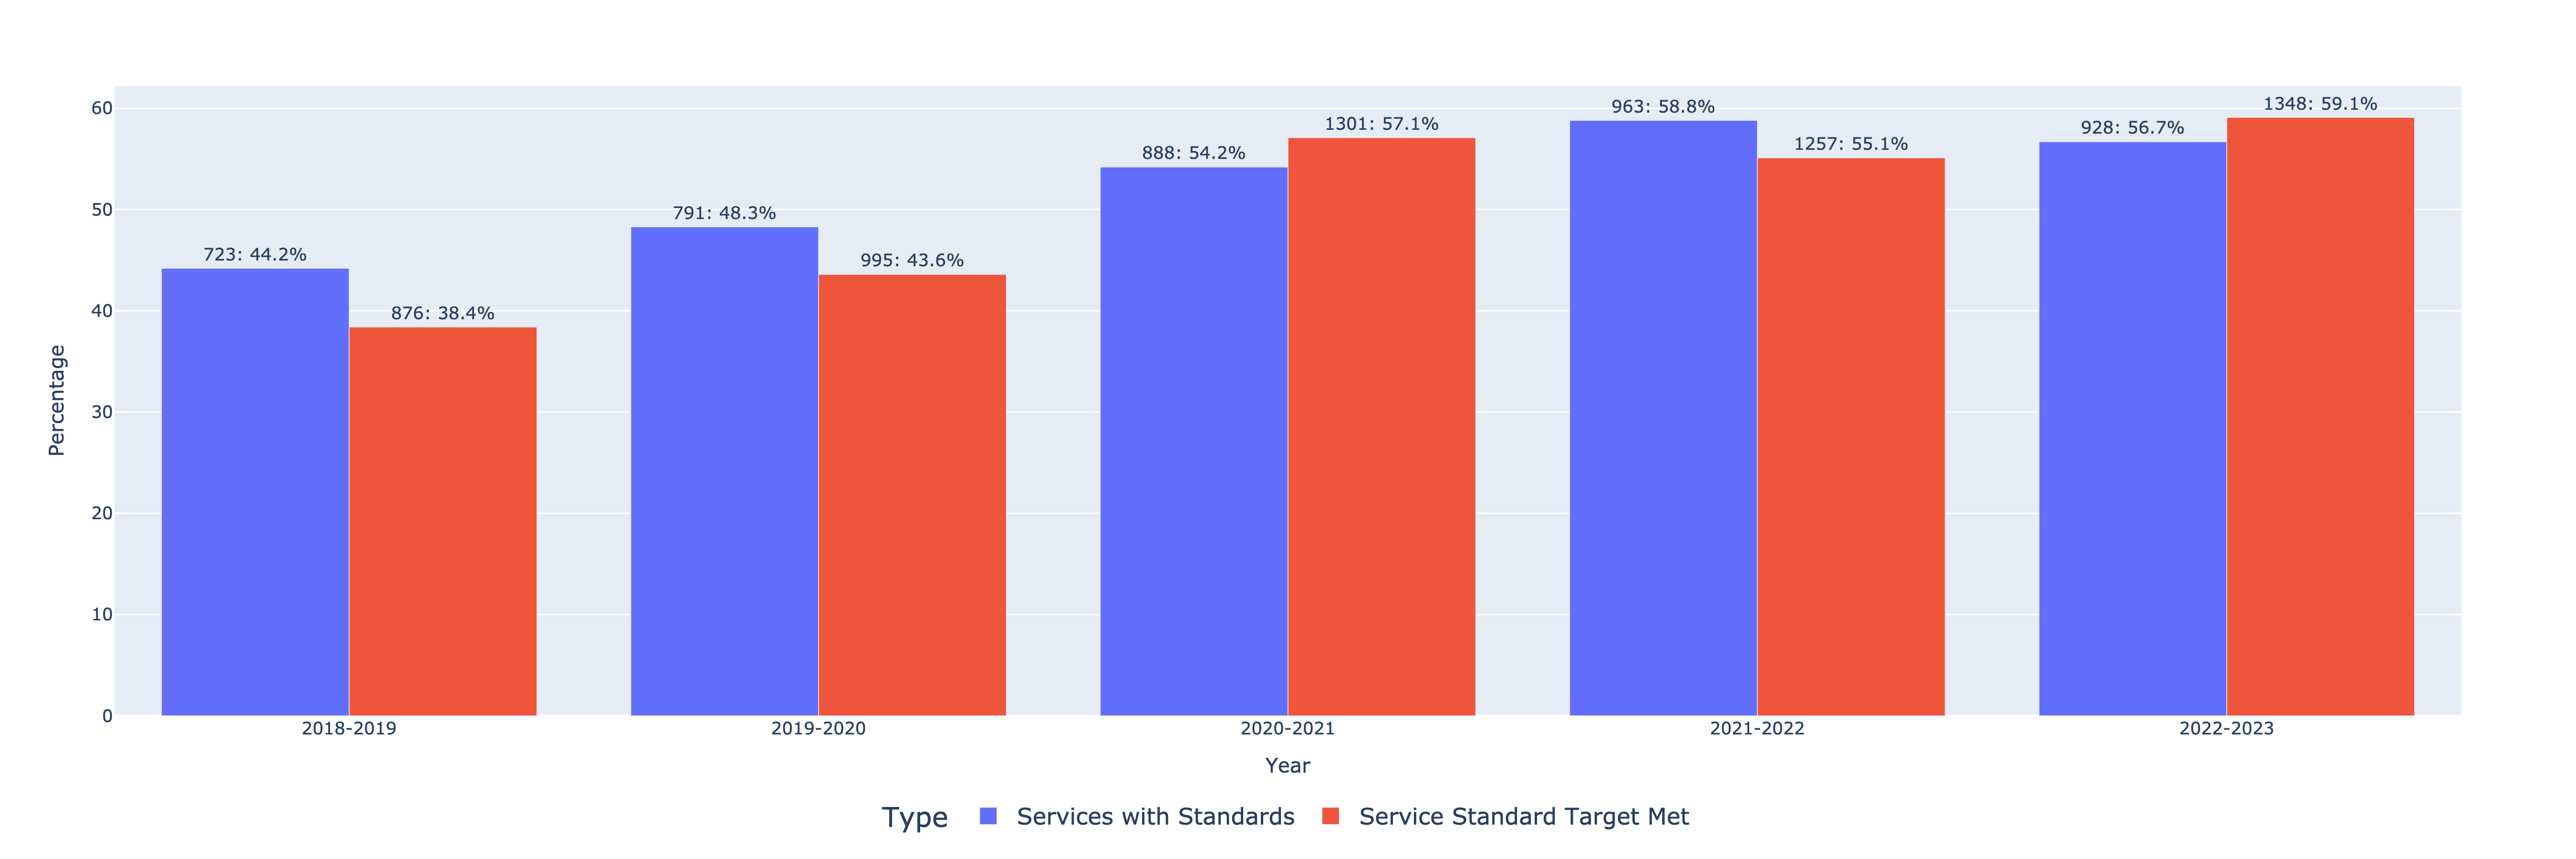
\includegraphics[width=1\linewidth]{StdWithTarget.png}
    \caption{\label{fig:Std}Percentage of Service with Standards and Standards with Target Met}
\end{figure}
